\documentclass{classrep}
\usepackage[utf8]{inputenc}

\usepackage[pdftex]{color,graphicx}
\DeclareGraphicsExtensions{.pdf,.png,.jpg,.bmp,.gif}

\usepackage{mathtools}
\usepackage{amsthm}
\usepackage{amsfonts}
\usepackage{float}
\usepackage{subfig}
\usepackage{color}
\usepackage{tabularx}
\usepackage{listings}
\usepackage{indentfirst}
\usepackage{color}
\usepackage{url}
\usepackage{hyperref}
\usepackage[polish]{babel}
\usepackage{paralist}
\usepackage{indentfirst}

\hypersetup{colorlinks=false,pdfborder={0 0 0}}

\definecolor{javared}{rgb}{0.6,0,0} % for strings
\definecolor{javagreen}{rgb}{0.25,0.5,0.35} % comments
\definecolor{javapurple}{rgb}{0.5,0,0.35} % keywords
\definecolor{javadocblue}{rgb}{0.25,0.35,0.75} % javadoc

\lstset{language=Java,
basicstyle=\ttfamily,
keywordstyle=\color{javapurple}\bfseries,
stringstyle=\color{javared},
commentstyle=\color{javagreen},
morecomment=[s][\color{javadocblue}]{/**}{*/},
numbers=left,
numberstyle=\tiny\color{black},
stepnumber=2,
numbersep=10pt,
tabsize=4,
showspaces=false,
showstringspaces=false}

\studycycle{Informatyka, studia dzienne, mgr II st.}
\coursesemester{I}

\coursename{Przetwarzanie obrazu i dźwięku}
\courseyear{2011/2012}

\courseteacher{dr inż. Arkadiusz Tomczyk}
\coursegroup{środa, 8:30}

\author{
  \studentinfo{Paweł Musiał}{178726} \and
  \studentinfo{Łukasz Michalski}{178724}
}
\title{Zadanie 4:\\  \textbf {Rozpoznawanie izolowanych słów w sygnale mowy.}}
\svnurl{https://serce.ics.p.lodz.pl/svn/labs/poid/at_sr0830/lmpm@}

\begin{document}
\maketitle

\addtocounter{footnote}{1}

\tableofcontents
\pagebreak
\section{Cel}
Realizacja zadania polega na stworzeniu aplikacji umożliwiającej obliczanie reprezentacji sygnału audio w~postaci ciągów wektorów współczynników MFCC i~porównywanie ich za pomocą algorytmu DTW. Należy stworzyć bazę zawierającą przynajmniej 10 różnych słów (przykładowo: ,,zero'', ,,jeden'', …, ,,dziewięć'') i~wykorzystać ją do rozpoznawania słowa wypowiedzianego przez użytkownika. W~celu poprawy wyników każde słowo zawarte w bazie może być reprezentowane przez kilka wzorców (np. nagranych przez różne osoby, albo w~różnych warunkach akustycznych).

Oprócz ostatecznego wyniku rozpoznania należy zaprezentować wyniki porównań dla wszystkich słów z bazy oraz tablice $g$ (preferowana metoda – w~postaci obrazu, reprezentującego wartości $g[i, j]$ za pomocą np. odcieni szarości). Należy rozważyć metodę modyfikacji algorytmu DTW pozwalającą na dopasowanie fragmentu słowa zamiast całości. Należy zaimplementować ograniczenia globalne zgodnie z~przydzielonym wariantem, przy czym powinna też istnieć możliwość wyłączenia tych ograniczeń, tak aby ścieżka mogła mieć dowolny kształt.
\begin{itemize}
\item Ograniczenie globalne typu Sakoe and Chiba band
\item \textbf{Ograniczenie globalne typu Itakura parallelogram}
\end{itemize}
\section{Wprowadzenie}
Rozpoznawanie mowy jest klasycznym problemem przetwarzania dźwięku, dla którego w ciągu minionych dziesięcioleci zaproponowano wiele rozwiązań. Wyróżniamy tu zasadniczo problem prostszy, polegający na rozpoznawaniu izolowanych słów oraz zadanie rozpoznawania mowy ciągłej. W obu przypadkach należy przyjąć założenia odnośnie sposobu reprezentacji i parametryzacji sygnału mowy oraz odnośnie metod dopasowania danych do wzorca w sposób niezależny od czasu trwania i zmian szybkości analizowanej wypowiedzi.
\subsection{MFCC (\textit{Mel-frequency cepstral coefficients})}
W trakcie procesu rozpoznawania mowy stosuje się różne metody reprezentowania widma amplitudowego sygnału wejściowego. Często wykorzystuje się tutaj reprezentacje w postaci tzw. cepstrum,i jego ponowne przekształcenie transformatą Fouriera lub cosinusową(„widmo widma”). Z tak powstałych współczynników wybiera się od kilku do kilkunastu (współczynniki cepstralne) , które opisują ogólną informacje o kształcie widma dźwięku. Stanowią one doskonałe narzędzie do późniejszej analizy i porównań dwóch sygnałów. Z uwagi na logarytmiczną zależność między częstotliwością dźwięku, a jego subiektywnie postrzeganą wysokością, dziedzinę częstotliwości, w której rozpatrywane jest widmo dźwięku należy przeskalować zgodnie z perceptualną skalą wysokości dźwięku (skalą melową)
przed powtórną transformatą Fouriera lub cosinową. Współczynniki cepstralne uzyskane w ten
sposób określamy właśnie jako MFCC.

\subsection{Algorytm DTW (\textit{Dynamic Time Warping})}
Metoda Dynamic Time Warping (\textit{DTW}) jest powszechnie wykorzystywana do porównywaniu ze sobą sygnałów różnej długości. Przeważnie znajduje zastosowanie w systemach rozpoznawania mowy, gdzie różnica~w prędkości wypowiadania danej głoski nie wpływa na znaczenie całego słowa.

Metoda \textit{DTW} pozwala na znalezienie najmniejszej odległości między dwoma szeregami czasowymi przy
dopuszczeniu przesunięć w czasie dla obu szeregów. Algorytm ten radzi sobie również w przypadku braku części danych lub ich niedokładności. Najważniejsza jest tutaj kolejność występowania poszczególnych faz szeregu czy sygnału. Dzięki takim właściwościom metoda \textit{DTW} doskonale nadaje się do rozpoznawania izolowanych słów.
\begin{figure}[h!]
\centering
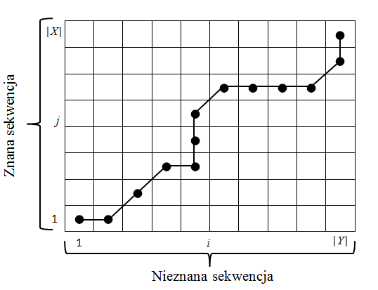
\includegraphics[width=10cm]{DTW.PNG} 
\caption{Ścieżka optymalnego dopasowania wyznaczona algorytmem \textit{DTW}.}
\label{fig:DTW}
\end{figure}
Porównywane metodą \textit{DTW} szeregi powinny być podzielone na ramki - momenty w jakich dokonywany był pomiar ich cech charakterystycznych. Obliczana jest bowiem macierz odległości między każdą ramką szeregu wejściowego i bazowego. Stosuje się w tym wypadku metrykę Euklidesową. Następnie trzeba wyliczyć macierz zakumulowanej odległości między próbkami (Rysunek \ref{fig:DTW}). Dla komórki [$i$, $j$] sumuję się z jej wartość z najmniejszą wartością jednej z trzech komórek sąsiednich [$i-1$,$j$], [$i$,$j-$] lub [$i-1$,$j-1$]. Całą operację zaczyna się od komórki [$0$,$0$]. Tak otrzymana macierz pozwala na wyznaczenie ścieżki optymalnego dopasowania do siebie tych dwóch szeregów.

Badając zmiany kierunku ścieżki można określi czy próbki te są do siebie podobne czy też różnią się. Istnieje wtedy nawet możliwość określenia momentu w którym różnica ta jest największa. Aby uznać, że dwie próbki reprezentują ten sam sygnał przyjmuje się kilka warunków jakie musi spełniać otrzymana ścieżka:
\begin{enumerate}
\item Jej przebieg musi być jak najbliższy diagonalnemu.
\item Ścieżka powinna poruszać się jedynie o jedno pole naraz. Eliminuje dziury czy braki dopasowań.
\item Ścieżka nie może zawracać. Jej kolejne współrzędne $i,j$ powinny pozostawać takie same lub rosnąc nigdy maleć.
\item Powinna zaczynać się w punkcie $[0,0]$ a kończyć $[i,j]$.
\item Ścieżka nie powinna też zbyt szybko lub zbyt wolno rosnąć. Ogranicza to możliwość dopasowania bardzo krótkich sekwencji do bardzo długich.
\end{enumerate}

Dodatkowo stosuje się się jeszcze tak zwane ograniczenia globalne nakładane na przebierz ścieżki optymalnego dopasowania. Najbardziej popularne są :
\begin{itemize}
\item Sakoe and Chiba band
\item Itakura parallelogram
\end{itemize}

Wykresy wyznaczonych obszarów dozwolonych przez te ograniczenia przedstawia rysunek \ref{fig:globalDTW}.

\begin{figure}[h!]
\centering
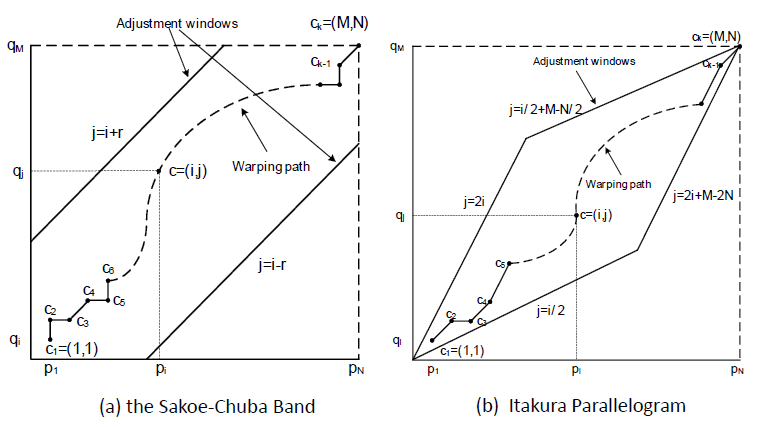
\includegraphics[width=12cm]{bands.PNG} 
\caption{Obszary dozwolone przez ograniczenia globalne.}
\label{fig:globalDTW}
\end{figure}

Stosując wszystkie te zasady można ograniczyć ilość możliwych ścieżek jakie da się wyznaczyć. Oznacza to, że wystarczy wtedy mniejsza liczba porównań aby określić czy dane próbki do siebie pasują. Nie spełnienie chociaż jednego z podanych tutaj warunków oznacza bowiem, że w pewnym momencie różnica między szeregami jest za duża. Przyspiesza to same operacje obliczeniowe i~skraca czas klasyfikacji próbki wejściowej do tych zapisanych~bazie.

\section{Opis implementacji}
\subsection{MFCC (\textit{Mel-frequency cepstral coefficients})}
Implementacja obliczania współczynników MFCC została oparta o algorytm podany w instrukcji do zadania 4b \cite{1}. Wykorzystaliśmy tutaj zewnętrzną bibliotekę do wyliczania współczynników FFT o nazwie jTransforms. Pozwala ona w sposób szybki i pewny wykonać przekształcenie przy pomocy algorytmu FFT. Dla zestawów filtrów w dziedzinie częstotliwości zbudowany w oparciu o skalę melową $H_{k}$ wartość współczynnika $K$ została dobrana i wynosi 40 natomiast wartość parametru $d$ jest dobierana adaptacyjne na podstawie wzoru \ref{wzor:MFCC}. Uzyskiwana ilość  współczynników MFCC na każdą ramkę wynosi 20. 
\begin{equation}\label{wzor:MFCC}
d=\frac{szerokoscOkna_{max}-szerokoscOkna_{min}}{K}
\end{equation}
,gdzie $K$ to ilość użytych filtrów.

\subsection{Algorytm DTW (\textit{Dynamic Time Warping})}
Podobnie jak obliczenia współczynników MFCC algorytm DTW został oparty o implementację opisaną w instrukcji do zadania 4b \cite{1}. Wartym przytoczenia tutaj jest kod reprezentujący obydwa ograniczenia globalne opisane w tym zadaniu:

Itakura parallelogram
\begin{lstlisting}
 public boolean check(int i, int j, int I, int J) {
        if (j > 2 * i) {
            return false;
        }
        if (j > i / 2 + I - J / 2) {
            return false;
        }
        if (j < 2 * i + I - 2 * J) {
            return false;
        }
        if (j < i / 2) {
            return false;
        }
        return true;
    }
\end{lstlisting}

oraz Sakoe and Chiba band
\begin{lstlisting}
  public boolean check(int i, int j, int I, int J) {
        return Math.abs((i * ((double) I / (double) J)) - j) <= r;
    }
\end{lstlisting}

Oba te ograniczenia zostały zaimplementowane w osobnych klasach implementujących wspólnie interfejs:
\begin{lstlisting}
public interface IGlobalConstraints {
    public boolean check(int i, int j , int I, int J);
}
\end{lstlisting}
Znaczenie poszczególnych parametrów funkcji \textit{check}:
\begin{itemize}
\item i,j - współrzędne badanego punktu ścieżki
\item I,J - długość sygnału wzorcowego i porównywanego
\end{itemize}

Dodatkowo w ramach zadania posłużyliśmy się algorytmem do usuwania ciszy przed i po wypowiedzianym słowie. Algorytm ten bazuje na pracy \cite{2} a jego implementacja pochodzi z \cite{3}. Mimo pozytywnych efektów jego niestety czasami pogarsza on rejestrowaną próbkę co utrudnia jej dopasowanie. Powód jego nieprawidłowej pracy mimo prób analizy nie został odkryty. Ze względu na to że pogorszenie występuje stosunkowo rzadko nie ma ono dużego wpływu na pracę całej aplikacji.

\section{Wyniki}

\section{Dyskusja}
W metodzie DTW duże znaczenie ma postać dostarczonych współczynników MFCC. Logarytmowanie podczas obliczania tych współczynników ma na celu uwydatnienie małych różnic, co w efekcie pozwala na lepsze rezultaty w odróżnianiu poszczególnych dźwięków. Dodatkowo aby odzwierciedlić percepcje ludzką w procesie ,,dopasowywania'' używana jest skala melowa, będąca logarytmiczna skalą odpowiadająca charakterystyce percepcji ludzkiej. Dzięki temu obiektywny wynik metody rozpoznawania słów, teoretycznie powinien lepiej odpowiadać naszemu subiektywnemu odczuciu podobieństwa testowanych słów. Teoretycznie, ponieważ w praktyce zadanie rozpoznawania słów nie jest zadaniem trywialnym. Opracowana przez nas metoda osiąga zadowalające wyniki, jednak jak wspomniano na początku, obliczane współczynniki MFCC mają duży wpływ na rezultat metody. Możliwym wydaje się, zatem lepszy wynik przy lepszym dostosowaniu sposobu obliczania współczynników MFCC.

\section{Wnioski}

\begin{thebibliography}{1}
\bibitem{1} Instrukcja do zadanie 4b \url{http://ftims.edu.p.lodz.pl/mod/resource/view.php?id=15798}
\bibitem{2} A New Silence Removal and Endpoint Detection Algorithm for Speech and Speaker Recognition Applications, G. Saha, Sandipan Chakroborty, Suman Senapati
\bibitem{3} Silence Removal and End Point Detection JAVA Code, Ganesh Tiwari \url{http://ganeshtiwaridotcomdotnp.blogspot.com/2011/08/silence-removal-and-end-point-detection_29.html}
\end{thebibliography}
\end{document}